\section{Evaluierung}
\label{sec5:eval}
In diesem Kapitel werden die Ergebnisse der Forschungsziele der vorangegangenen Phasen
\begin{itemize}
  \item Beobachtungsphase, \cref{sec2:sota} \enquote{Stand der Wissenschaft und Technik}
  \item Theoriebildungsphase, \cref{sec3:model} \enquote{Modellierung}
  \item Implementierungsphase, \cref{sec4:impl} \enquote{Implementierung}
\end{itemize}
im Vergleich zu den in \cref{sec1:intro:subsec:research-questions} identifizierten, initialen Forschungsfragen in einer detaillierten Evaluierung überprüft.
Ziel der Evaluierung ist es, Erkenntnisse zur Vollständigkeit, sowie Korrektheit der prototypischen Software für die Prototypen der Benutzungsschnittstelle(n) und Funktionen der Anwendung zu erlangen.
Dieses Ziel ergibt sich aus der in diesem Kapitel gewählten Methodik der Evaluierung, sowie aus den Forschungszielen vom Typ Experiment und folgt dem Ansatz nach Nunamaker \cite{nunamaker}.
Zudem werden konkrete Ziele der Evaluierung, Auswahl von Methoden der Evaluierung, um diese Ziele zu erreichen, sowie die Vorbereitung, Durchführung und Auswertung von Experimenten nach den gewählten Methoden der Evaluierung, beschrieben.
Mit diesem Ansatz werden alle Problembereiche im Vergleich zu den initialen Forschungszielen zufriedenstellend und ausführlich abgedeckt.

Die Gliederung des Kapitels lautet wie folgt:
\cref{sec5:eval:subsec:eval-goals-methodology} konkretisiert die Ziele und zu beantwortenden Fragestellungen der Evaluierung.
Des Weiteren wird für die Evaluierung eine geeignete Evaluierungsmethodik gewählt und erläutert.
In \cref{sec5:eval:subsec:assign-exper} werden die in der Evaluierung durchzuführenden Experimente formuliert, sowie den entsprechenden Forschungszielen zugeordnet.
In \cref{sec5:eval:subsec:fz-explainability,sec5:eval:subsec:fz-integration} werden jeweils die Vorbereitung, Durchführung und die Ergebnisse der jeweiligen Experimente beschrieben.
In \cref{sec5:eval:subsec:adaptation} werden in Abhängigkeit der in den Experimenten potentiell entdeckten Mängel, Fehlerbehandlungen beschrieben.
In \cref{sec5:eval:subsec:summary} werden dann die Ergebnisse der Evaluierung zusammengefasst und diskutiert.

\subsection[Ziele der Evaluierung und geeignete Evaluierungsmethodik]{\texorpdfstring{Ziele der Evaluierung und geeignete \\ Evaluierungsmethodik}{Ziele der Evaluierung und geeignete Evaluierungsmethodik}}
\label{sec5:eval:subsec:eval-goals-methodology}
Wesentliches Ziel der Evaluierung ist die Sicherstellung der Funktionalität der entwickelten, prototypischen Proof-of-Concept Implementierung.
In diesem Abschnitt werden die konkreten Ziele der Evaluierung formuliert, auf deren Basis eine geeignete Evaluierungsmethodik ausgewählt wird.
Konkrete Ziele lassen sich aus den Forschungszielen vom Typ Experiment ableiten.
Folgende konkrete Ziele können dabei formuliert werden:
Bewertung der \undline{Vollständigkeit} und \undline{Korrektheit} der prototypischen Proof-of-Concept Implementierung in Bezug auf die in \cref{sec3:model} \enquote{Modellierung} entwickelten Konzepte.
Diese Ziele stellen die Grundlage für die Auswahl einer Evaluierungsmethodik dar.
Durch Gruppierung und Zuweisung dieser Ziele zu einem Experiment können mehrere Ziele in einer Durchführung eines Experiments abgedeckt werden.
Aus diesen festgelegten, konkreten Zielen ergibt sich folgendes Ziel der Evaluierung, für dessen Erreichen Experimente entworfen werden, die nach ihrer Durchführung Erkenntnisse bezüglich der Vollständigkeit und Korrektheit der prototypischen Proof-of-Concept Implementierung der Software zulassen.

In \cref{sec2:sota:subsec:eval-methodology} wurden Methodiken vorgestellt, mit welchen eine systematische Evaluierung einer Anwendung möglich ist.
Mittels dieser Methodiken können Aussagen und Bewertungen zur entwickelten Software vorgenommen werden.
Es gilt aus der Sammlung dieser Methodiken eine geeignete Methodik zu wählen, die mit den in diesem Projekt begrenzten Ressourcen und Möglichkeiten zur Verfügung stehen und mit welcher möglichst viele formulierten Ziele erreicht werden können.
Ein weiterer wichtiger Aspekt, den es bei der Auswahl eines geeigneten Evaluierungsverfahrens bzw. -methodik zu beachten gilt, ist, dass es sich bei der zu evaluierenden Software nicht um ein fertiges, einsetzbares Softwareprodukt handelt, sondern nur um eine prototypische Proof-of-Concept Implementierung.
Da im Rahmen der Implementierung ein praktisch, benutzbarer Softwareprototyp entwickelt wurde, bietet es sich an, genau diesen Prototyp zur Evaluierung zu verwenden, sodass sich die Erkenntnisse und Ergebnisse der Evaluierung auf den aktuellsten Stand der Software und somit auch dieser Arbeit beziehen.

% Für die Durchführung kann auf einen Experten zurückgegriffen werden... (S.W.)
Für die Durchführung der Evaluierung kann auf einen Experten des Lehrgebiets Multimedia und Internetanwendungen zurückgegriffen werden.
Aus den verfügbaren Evaluierungsmethodiken wird im Folgenden der Cognititve Walkthrough gewählt.
Der Cognititve Walkthrough generiert keine Erkenntnisse bezüglich der Effektivität einer Anwendung, bietet sich jedoch trotzdem zur Evaluierung an, da dieser einfach, kostengünstig und mit limitierten Ressourcen durchführbar ist.
Im Verfahren des Cognititve Walkthrough werden systematisch atomare Aktionen durchlaufen.
Diese atomaren Aktionen sind Aufgaben, die ein Benutzer ausführen muss, um sein angestrebtes Ziel zu erreichen, und lassen sich aus den entsprechenden Interaktionen eines Benutzers mit dem System, festgehalten in \cref{sec3:model:par:mechanism-use-cases} \enquote{Anwendungsfällen}, ableiten.
Mit diesem Vorgehen wird sich versprochen, gezielt Erkenntnisse zu den Zielen \enquote{Bewertung der Vollständigkeit und Korrektheit} zu erlangen.
Andere umfangreichere Evaluierungsmethodiken sind im Rahmen dieser Arbeit nicht anwendbar aufgrund mangelnder zeitlicher, sowie personeller Ressourcen.

Im weiteren Verlauf dieses Kapitels wird ein Cognititve Walkthrough geplant, in seiner Durchführung beschrieben und schlussendlich anhand der gewonnenen Erkenntnisse ausgewertet.
Ziel der Durchführung eines Cognititve Walkthrough ist es, neue Erkenntnisse zur Funktionalität der entwickelten Anwendung durch Bewertung der Vollständigkeit und Korrektheit zu erlangen.
Hierfür wird im nächsten Abschnitt eine Wahl und Zuweisung der in der Evaluierung durchzuführenden Experimente vorgenommen.

\subsection{Wahl und Zuweisung durchzuführender Experimente}
\label{sec5:eval:subsec:assign-exper}
In Vorbereitung des Cognitive Walkthroughs werden aus den in \cref{sec3:model:par:mechanism-use-cases} beschriebenen Anwendungsfällen zwei Experimente abgeleitet, deren Durchführung evaluiert werden soll und die durch Funktionen der Anwendung unterstützt werden.
Diese Experimente lauten wie folgt:

\begin{enumerate}
  \item \textbf{Exp. 1}: Interaktion mit Graph Codes.

  % UC-1.1, 1.2, 1.3, 1.4, 1.5
  Im Rahmen dieses Experiments interagiert der Experte unter Nutzung der Benutzungsschnittstelle der Anwendung mit Graph Codes.
  Interaktionen umfassen das Importieren, Entfernen und Verarbeiten von Graph Codes.
  Durch dieses Experiment werden die Anwendungsfälle UC-1.1 bis 1.6 abgedeckt.

  \item \textbf{Exp. 2}: Erstellen einer Erklärung.

  % UC-1.6, 1.7, 1.8
  Im Rahmen dieses Experiments erstellt der Experte unter Nutzung der Benutzungsschnittstelle anhand eines vorher ausgewählten Graph Codes eine textuelle oder visuelle Erklärung.
  Wichtige Voraussetzung für dieses Experiments ist somit das erste Experiment \textbf{Exp. 1}.
  Durch dieses Experiment werden die Anwendungsfälle UC-1.6 bis 1.8 abgedeckt.
\end{enumerate}

Experiment \textbf{Exp. 1} wird durch das Forschungsziel \enquote{FZ 1.4/E Erklärbarkeit von MMIR mittels generativer KI} in \cref{sec5:eval:subsec:fz-explainability} durchgeführt und beschrieben.
Analog wird Experiment \textbf{Exp. 2} durch das Forschungsziel \enquote{FZ 2.4/E Integration generativer KI in das GMAF} in \cref{sec5:eval:subsec:fz-integration} durchgeführt und beschrieben.

\clearpage

\subsection[FZ 1.4/E Erklärbarkeit von MMIR mittels generativer KI]{\texorpdfstring{FZ 1.4/E Erklärbarkeit von MMIR mittels \\ generativer KI}{FZ 1.4/E Erklärbarkeit von MMIR mittels generativer KI}}
\label{sec5:eval:subsec:fz-explainability}
In diesem Abschnitt bzw. Forschungsziel wird das Experiment \textbf{Exp. 1} behandelt.
In \cref{sec5:eval:subsubsec:exp-1:preparation} wird die Vorbereitung des Cognitive Walkthroughs und in \cref{sec5:eval:subsubsec:exp-1:execution} die Durchführung des Cognitive Walkthroughs beschrieben.
Schlussendlich werden in \cref{sec5:eval:subsubsec:exp-1:results-discussion} dann die Ergebnisse der Durchführung, wie z.B. entdeckte Mängel festgehalten und Fehlerbehandlungen beschrieben.

% Experiment 1

\subsubsection{Vorbereitung}
\label{sec5:eval:subsubsec:exp-1:preparation}
Die Vorbereitung des Cognitive Walkthroughs beinhaltet den Aufbau einer adäquaten Kollektion an Graph Code Dateien.
Für diese Graph Code Dateien ist wiederum eine geeignete Kollektion an Multimediainhalten notwendig.
Das GMAF bietet hierfür bereits eine Kollektion an Multimediainhalten bzw. Graph Code Dateien in einem dafür dedizierten Ordner \enquote{/graphcodes} an.

Ein wichtiger Teil für die Vorbereitung eines Cognitive Walkthroughs ist die Beschreibung der Aktionssequenz, die den Ablauf atomarer Aktionen auflistet, die ein Benutzer zur Lösung einer Aufgabe abarbeiten muss.
Die Aktionssequenz für das Experiment \textbf{Exp. 1}.

\begin{tcolorbox}[minipage, colback=white, colframe=black, arc=0pt, outer arc=0pt]
  \begin{enumerate}
    \setlength{\itemsep}{1pt}
    \item Starten der Anwendung, Modul Explainer auswählen und starten.
    \item Importieren von Graph Code(s) durch Mausklick auf den Knopf \enquote{Import Graph Code(s)}.
    \item Auswahl von Graph Code(s) aus der Liste in der Benutzungsschnittstelle \enquote{GraphCode - Editor}.
    \tcbline
    \item[] Ab hier kann zwischen zwei weiteren Interaktionen in einer Fallunterscheidung differenziert werden.
    \tcbline
    \setcounter{enumi}{3}
    \item Fall 1: Entfernen der ausgewählten Graph Code(s) durch Mausklick auf den Knopf \enquote{Remove selected Graph Code(s)}.
    \item Fall 2: Ausführen einer Operation auf den ausgewählten Graph Code(s).
    \begin{enumerate}[label*=\arabic*.]
      \item Auswahl einer Operation in einer ein- und ausklappbaren Liste.
      \item Ausführen der ausgewählten Operation auf den ausgewählten Graph Codes durch Mausklick auf den Knopf \enquote{Execute}.
    \end{enumerate}
    \item Ggfs. Wiederholung der Schritte 2 bis 5 oder 3 bis 5.
  \end{enumerate}
\end{tcolorbox}

Diese Aktionssequenz ist die Grundlage für die folgende Durchführung des Experiments \textbf{Exp. 1}.
Hierbei wird jede atomare Aktion aus der Aktionssequenz durchgeführt und durch einen Expertennutzer analysiert.

Eine weitere, wichtige Aufgabe im Rahmen der Vorbereitung dieses Experiments ist die Beschreibung der Gruppe zu erwartender Anwender bzw. Benutzer.
Aufgrund der Tatsache, dass die Anwendung \enquote{Explainer} ein Modul bzw. Teil des GMAF ist, können Rückschlüsse auf mögliche Benutzergruppen getroffen werden.
Daher wird angenommen, dass ein typischer Benutzer der Anwendung mindestens durchschnittlich erfahren mit der Bedienung von Computersystemen im Allgemeinen ist und darüber hinaus ebenfalls Kenntnisse über Funktionen und der Bedienung (kommerzieller) Programme bzw. Systeme zur Text- und Bildgenerierung besitzt.
Zwecks der Validierung der Funktionalität des Moduls wird weiterhin angenommen, dass ein typischer Benutzer des Moduls nur über wenig Erfahrung im Umgang mit diesem Modul besitzt.
Weitere, speziellere Kenntnisse werden nicht erwartet, oder vorausgesetzt.

Zum Abschluss der Vorbereitung werden eine Reihe an potentiellen Zielen festgehalten, die ein Benutzer des GMAF beim Start der Aufgabe bzw. einer Variation dieser erfüllen will.
Eine Variation der ersten Aufgabe könnte hierbei das Bestimmen der Gemeinsamkeiten der Merkmale aus einer Kollektion an Multimediainhalten sein.

\begin{tcolorbox}[minipage, colback=white, colframe=black, arc=0pt, outer arc=0pt]
  Bestimme die Gemeinsamkeiten der Merkmale aus einer Kollektion an Multimediainhalten.
  \begin{itemize}
    \item[$\mapsto$] Starte die Benutzeroberfläche des Moduls Explainer.
    \begin{itemize}
      \item[$\mapsto$] Wähle und importiere eine Reihe an Graph Codes aus der Kollektion aus.
      \item[$\mapsto$] Wähle eine Operation, in diesem Fall Gemeinsamkeiten, aus und führe diese aus.
    \end{itemize}
  \end{itemize}
\end{tcolorbox}

Damit ist die Vorbereitung des Cognitive Walkthroughs zur ersten Aufgabe abgeschlossen und in den folgenden Abschnitten werden die Durchführung, sowie die aus dieser Durchführung erschlossenen Ergebnisse vorgestellt, beschrieben und in einer Diskussion eingeordnet.

\subsubsection{Durchführung}
\label{sec5:eval:subsubsec:exp-1:execution}
Der in dieser Durchführung beschriebene Cognitive Walkthrough wurde in einer Live-Video-Sitzung am 16.10.2023 durchgeführt.
An dieser Sitzung nahmen Jens Nathan Andreß, der Autor dieser Arbeit und Prof. Dr.-Ing. Stefan Wagenpfeil, der Betreuer dieser Bachelorarbeit, teil.
Anstelle eines formalen Cognitive Walkthroughs als Evaluierungsmethodik wird in der Durchführung eine informelle Variante des Cognitive Walkthroughs angewandt.
Diese informelle Variante der Evaluierungsmethodik zeichnet sich dadurch aus, dass der Experte die in der Vorbereitung beschriebene Aktionssequenz schrittweise bearbeitet und das Verhalten eines Benutzers simuliert bzw. nachempfindet.
Anders als bei einem formalen Cognitive Walkthrough mit einem vorher angefertigten Fragenkatalog für jede in der Aktionssequenz definierte Aktion, werden in dieser Durchführung die Aussagen des Expertennutzers zu den jeweiligen Aktionen informell schriftlich festgehalten.
Diese Aussagen können insbesondere potentiell auftretende Probleme umfassen, mit denen sich ein nachempfundener Benutzer konfrontiert sehen könnte.
In Bezug auf die bereits ohnehin schon eingeschränkten zeitlichen und personellen Ressourcen muss daher mit qualitativen Abzügen bei den durch diesen informellen Durchlauf gesammelten Erkenntnissen gerechnet werden.
Nichtsdestotrotz können mit dieser informellen Variante und den begrenzten Ressourcen in dieser Arbeit, die in \cref{sec5:eval:subsec:eval-goals-methodology} definierten Ziele zufriedenstellend erreicht werden.
Prof. Dr.-Ing. Stefan Wagenpfeil nahm während der Sitzung die Rolle des Experten an und imitierte das Verhalten eines Benutzers aus der in der Vorbereitung angenommenen Benutzergruppe und machte Anmerkungen zu den jeweils durchgeführten Aktionen aus der Aktionssequenz, die in der folgenden Beschreibung der Durchführung hervorgehoben werden.
Zudem werden ggfs. ausgewählte Schritte der Aktionssequenz mit Bildschirmaufnahmen relevanter Ausschnitte der jeweiligen Benutzungsschnittstelle dokumentiert.

Die Durchführung des ersten Experiments \textbf{Exp. 1} beginnt mit der ersten Aktion in der Aktionssequenz, dem Starten der GMAF-Anwendung und dem Auswählen des Moduls \enquote{Explainer}.
% Experte merkt an, dass das Fenster in welchem das Modul sitzt aufgrund der in den Komponenten dargestellten, zu antizipierenden Inhalten zu klein ist und standardmäßig maximiert sein soll
Der Experte merkt an, dass das Fenster, in welchem sich das Modul öffnet, aufgrund der in den Komponenten dargestellten, zu antizipierenden Inhalten zu klein ist.
Eine mögliche Anpassung der Benutzungsschnittstelle wird im nachfolgenden \cref{sec5:eval:subsubsec:exp-1:results-discussion} besprochen.
Nach dem Starten des Moduls sieht sich der Benutzer mit der in \cref{sec4:impl:subsubsec:summary-findings:fig:ui-ex-1} dargestellten Benutzungsschnittstelle konfrontiert.

In Schritt 2 der Aktionssequenz klickt der Benutzer durch einen Mausklick auf den Knopf \enquote{Import Graph Code(s)}.
Daraufhin wird dem Benutzer ein systemweiter Auswahldialog zum Auswählen von Dateien, genauer Graph Code Dateien angezeigt.
Dieser Dialog verweist bereits auf den in der Vorbereitung angemerkten, für die Kollektion an Graph Codes dedizierten Ordner im GMAF.
Aus diesem Auswahldialog wählt der Benutzer ein oder mehrere Graph Code Datei(en) aus.
Diese ausgewählten Graph Code Dateien werden dann in der Benutzungsschnittstelle \enquote{GraphCode - Editor} einer Liste hinzugefügt und angezeigt.
Der Experte stellt fest, dass dies der Erwartungshaltung eines Benutzers aus der in der Vorbereitung definierten Benutzergruppe entspricht.
Durch diese Reihe an Aktionen wird der Anwendungsfall \hyperref[sec3:model:uc-1.1]{UC-1.1} abgedeckt.

In Schritt 3 der Aktionssequenz wählt der Benutzer aus der Liste in der Benutzungsschnittstelle \enquote{GraphCode - Editor} ein oder mehrere Graph Code(s) aus.
Die Auswahl eines Graph Codes in der Liste wird dem Benutzer standardmäßig durch das visuelle Hervorheben des ausgewählten Elements bestätigt (siehe \cref{sec4:impl:par:ui-elements:fig:wireframe-ui-left-complete}).
Darüber hinaus werden durch die Auswahl eines Graph Codes aus der Liste andere Benutzungsschnittstellen beeinflusst, die dem Benutzer die Wirkung der Auswahl verdeutlichen.
Der Experte stellt fest, dass dies der Erwartungshaltung eines Benutzers aus der in der Vorbereitung definierten Benutzergruppe entspricht.
Durch diese Aktion wird der Anwendungsfall \hyperref[sec3:model:uc-1.3]{UC-1.3} abgedeckt.

In Schritt 4 der Aktionssequenz klickt der Benutzer durch einen Mausklick auf den Knopf \enquote{Remove selected Graph Code(s)}.
Daraufhin werden die bereits in der Liste ausgewählten Graph Codes aus dieser entfernt.
Der Experte stellt fest, dass dies der Erwartungshaltung eines Benutzers aus der in der Vorbereitung definierten Benutzergruppe entspricht.
Durch diese Aktion wird der Anwendungsfall \hyperref[sec3:model:uc-1.2]{UC-1.2} abgedeckt.

In Schritt 5 der Aktionssequenz führt der Benutzer eine Operation auf den in der Liste ausgewählten Graph Codes aus.
Hierfür trifft der Benutzer in einer Unteraktion eine Auswahl bezüglich der auszuführenden Operation auf den ausgewählten Graph Codes.
Der Experte stellt fest, dass die Benutzungsschnittstelle zur Auswahl der Operation nur die Namen der Operationen auflistet, es aber nicht erkenntlich ist, dass es sich dabei um Operationen auf Graph Codes handelt (siehe \cref{sec4:impl:par:ui-elements:fig:wireframe-ui-4}).
Es ist daher möglich, dass dem Benutzer nicht ersichtlich ist, dass es sich dabei um eine Operation auf Graph Codes handelt.
Eine mögliche Anpassung der Benutzungsschnittstelle wird im nachfolgenden \cref{sec5:eval:subsubsec:exp-1:results-discussion} besprochen.
In einer weiteren Unteraktion klickt der Benutzer durch einen Mausklick auf den Knopf \enquote{Execute}.
Daraufhin wird die ausgewählte Operation auf den in der Liste ausgewählten Graph Codes ausgeführt.
Der Experte hält fest, dass die Ergebnisse der ausgeführten Operationen augenscheinlich korrekt sind und dies der Erwartungshaltung eines Benutzers aus der in der Vorbereitung definierten Benutzergruppe entspricht.
Durch diese Aktionen werden die Anwendungsfälle \hyperref[sec3:model:uc-1.4]{UC-1.4} und \hyperref[sec3:model:uc-1.5]{UC-1.5} abgedeckt.

Im nächsten Abschnitt werden die aus dieser Durchführung gewonnenen Erkenntnisse aufgezählt, diskutiert und mögliche Anpassungen der Benutzungsschnittstelle besprochen.

\subsubsection{Ergebnisse und Diskussion}
\label{sec5:eval:subsubsec:exp-1:results-discussion}
Das Ergebnis des im vorigen Abschnitts durchgeführten Experiments unter der Anwendung des Cognitive Walkthroughs als Evaluierungsmethodik ist eine Liste an Mängeln, die in der prototypischen Software entdeckt werden konnten.
In diesem Abschnitt werden die entdeckten Mängel aufgezählt, beschrieben und es wird jeweils ein Lösungsansatz vermerkt, mit welchem der entsprechende Mangel abgestellt werden kann.

\undline{\textbf{Mangel 1:}}
Das Fenster, in welchem die Benutzungsschnittstelle dargestellt wird, ist zu klein.

Der Mangel kann behoben werden, indem das Fenster für die Benutzungsschnittstelle beim Starten des Moduls maximiert dargestellt wird.

\undline{\textbf{Mangel 2:}}
Dem Benutzer ist nicht ersichtlich, dass es sich bei den in der Auswahlliste angebotenen Elementen um gleichnamige Operationen auf Graph Codes handelt.

Der Mangel kann behoben werden, indem der Auswahlliste an der ersten Position ein Element \enquote{Graph Code Operation} hinzugefügt wird.

Nach Durchführung des Experiments und dem Beschreiben der identifizierten Mängel kann festgehalten werden, dass die getesteten Funktionen der Anwendung vollständig und korrekt umgesetzt wurden.
Als solches wurden beide formulierten Ziele, die Ziele der Vollständigkeit und der Korrektheit zufriedenstellend erfüllt bzw. abgedeckt.

\clearpage

\subsection{FZ 2.4/E Integration generativer KI in das GMAF}
\label{sec5:eval:subsec:fz-integration}
In diesem Abschnitt bzw. Forschungsziel wird das Experiment \textbf{Exp. 2} behandelt.
In \cref{sec5:eval:subsubsec:exp-2:preparation} wird die Vorbereitung des Cognitive Walkthroughs und in \cref{sec5:eval:subsubsec:exp-2:execution} die Durchführung des Cognitive Walkthroughs beschrieben.
Schlussendlich werden in \cref{sec5:eval:subsubsec:exp-2:results-discussion} dann die Ergebnisse der Durchführung, wie z.B. entdeckte Mängel festgehalten und Fehlerbehandlungen beschrieben.

% Experiment 2

\subsubsection{Vorbereitung}
\label{sec5:eval:subsubsec:exp-2:preparation}
Die Vorbereitung des Cognitive Walkthroughs beinhaltet den Aufbau einer adäquaten Kollektion an Graph Code Dateien.
Für diese Graph Code Dateien ist wiederum eine geeignete Kollektion an Multimediainhalten notwendig.
Das GMAF bietet hierfür bereits eine Kollektion an Multimediainhalten bzw. Graph Code Dateien in einem dafür dedizierten Ordner \enquote{/graphcodes} an.

Ein wichtiger Teil für die Vorbereitung eines Cognitive Walkthroughs ist die Beschreibung der Aktionssequenz, die den Ablauf atomarer Aktionen auflistet, die ein Benutzer zur Lösung einer Aufgabe abarbeiten muss.
Die Aktionssequenz für das Experiment \textbf{Exp. 2}.

\begin{tcolorbox}[minipage, colback=white, colframe=black, arc=0pt, outer arc=0pt]
  \begin{enumerate}
    \setlength{\itemsep}{1pt}
    \item Starten der Anwendung, Modul Explainer auswählen.
    \item Importieren von Graph Code(s) durch Mausklick auf den Knopf \enquote{Import Graph Code(s)}.
    \item Auswahl eines Graph Codes aus der Liste in der Benutzungsschnittstelle \enquote{GraphCode - Editor}.
    \item Erklärungstyp (Image / Text) in der Benutzungsschnittstelle \enquote{GraphCode - Explanation} auswählen.
    \item Anfrage mittels erweiterten Optionen parametrisieren.
    \item Generieren einer Erklärung durch Mausklick auf den Knopf \enquote{Generate ...}.
  \end{enumerate}
\end{tcolorbox}

Diese Aktionssequenz ist die Grundlage für die folgende Durchführung des Experiments \textbf{Exp. 2}.
Hierbei wird jede atomare Aktion aus der Aktionssequenz durchgeführt und analysiert.

Eine weitere, wichtige Aufgabe im Rahmen der Vorbereitung dieses Experiments ist die Beschreibung der Gruppe zu erwartender Anwender bzw. Benutzer.
Aufgrund der Tatsache, dass die Anwendung \enquote{Explainer} ein Modul bzw. Teil des GMAF ist, können Rückschlüsse auf mögliche Benutzergruppen getroffen werden.
Daher wird angenommen, dass ein typischer Benutzer der Anwendung mindestens durchschnittlich erfahren mit der Bedienung von Computersystemen im Allgemeinen ist und darüber hinaus ebenfalls Kenntnisse über Funktionen und der Bedienung (kommerzieller) Programme bzw. Systeme zur Text- und Bildgenerierung besitzt.
Zwecks der Validierung der Funktionalität des Moduls wird weiterhin angenommen, dass ein typischer Benutzer des Moduls nur über wenig Erfahrung im Umgang mit diesem Modul besitzt.
Weitere, speziellere Kenntnisse werden nicht erwartet, oder vorausgesetzt.

Zum Abschluss der Vorbereitung werden eine Reihe an potentiellen Zielen festgehalten, die ein Benutzer des GMAF beim Start der Aufgabe erfüllen will.

\begin{tcolorbox}[minipage, colback=white, colframe=black, arc=0pt, outer arc=0pt]
  Generiere eine Erklärung zu einem ausgewählten Graph Code.
  \begin{itemize}
    \item[$\mapsto$] Starte die Benutzeroberfläche des Moduls Explainer.
    \begin{itemize}
      \item[$\mapsto$] Wähle und importiere eine Reihe an Graph Codes aus der Kollektion aus.
      \item[$\mapsto$] Wähle einen Graph Code, zu welchem eine Erklärung generiert werden soll, aus.
      \item[$\mapsto$] Wähle einen Erklärungstyp (Image / Text) aus.
      \item[$\mapsto$] Starte die Generierung einer Erklärung.
    \end{itemize}
  \end{itemize}
\end{tcolorbox}

Damit ist die Vorbereitung des Cognitive Walkthroughs zur ersten Aufgabe abgeschlossen und in den folgenden Abschnitten werden die Durchführung, sowie die aus dieser Durchführung erschlossenen Ergebnisse vorgestellt, beschrieben und in einer Diskussion eingeordnet.

\subsubsection{Durchführung}
\label{sec5:eval:subsubsec:exp-2:execution}
Der in dieser Durchführung beschriebene Cognitive Walkthrough wurde in einer Live-Video-Sitzung am 16.10.2023 durchgeführt.
An dieser Sitzung nahmen Jens Nathan Andreß, der Autor dieser Arbeit und Prof. Dr.-Ing. Stefan Wagenpfeil, der Betreuer dieser Bachelorarbeit, teil.
Anstelle eines formalen Cognitive Walkthroughs als Evaluierungsmethodik wird in der Durchführung eine informelle Variante des Cognitive Walkthroughs angewandt.
Diese informelle Variante der Evaluierungsmethodik zeichnet sich dadurch aus, dass der Experte die in der Vorbereitung beschriebene Aktionssequenz schrittweise bearbeitet und das Verhalten eines Benutzers simuliert bzw. nachempfindet.
Anders als bei einem formalen Cognitive Walkthrough mit einem vorher angefertigten Fragenkatalog für jede in der Aktionssequenz definierte Aktion, werden in dieser Durchführung die Aussagen des Expertennutzers zu den jeweiligen Aktionen informell schriftlich festgehalten.
Diese Aussagen können insbesondere potentiell auftretende Probleme umfassen, mit denen sich ein nachempfundener Benutzer konfrontiert sehen könnte.
In Bezug auf die bereits ohnehin schon eingeschränkten zeitlichen und personellen Ressourcen muss daher mit qualitativen Abzügen bei den durch diesen informellen Durchlauf gesammelten Erkenntnissen gerechnet werden.
Nichtsdestotrotz können mit dieser informellen Variante und den begrenzten Ressourcen in dieser Arbeit, die in \cref{sec5:eval:subsec:eval-goals-methodology} definierten Ziele zufriedenstellend erreicht werden.
Prof. Dr.-Ing. Stefan Wagenpfeil nahm während der Sitzung die Rolle des Experten an und imitierte das Verhalten eines Benutzers aus der in der Vorbereitung angenommenen Benutzergruppe und machte Anmerkungen zu den jeweils durchgeführten Aktionen aus der Aktionssequenz, die in der folgenden Beschreibung der Durchführung hervorgehoben werden.
Zudem werden ggfs. ausgewählte Schritte der Aktionssequenz mit Bildschirmaufnahmen relevanter Ausschnitte der jeweiligen Benutzungsschnittstelle dokumentiert.

Die ersten Schritte 1 bis 3 der Aktionssequenz verhalten sich analog zu denen in \textbf{Exp. 1}.
Als solches werden die in diesen Schritten gewonnenen Erkenntnisse im nachfolgenden \cref{sec5:eval:subsubsec:exp-2:results-discussion} nicht berücksichtigt.

In Schritt 4 der Aktionssequenz wählt der Benutzer in der Benutzungsschnittstelle \enquote{GraphCode - Explanation} einen Erklärungstypen, \enquote{Image} oder \enquote{Text} aus.
Daraufhin wird dem Benutzer, in Abhängigkeit des jeweiligen Erklärungstypen, jeweils eine spezifische Benutzungsschnittstelle zum Erstellen einer entsprechenden Erklärung für einen ausgewählten Graph Code angezeigt (siehe \cref{sec4:impl:subsubsec:summary-findings:fig:ui-ex-1,sec4:impl:subsubsec:summary-findings:fig:ui-ex-2}).
Der Experte hat zwei Anmerkungen in Bezug auf die Benutzungsschnittstelle, speziell auf das Textfeld \enquote{Generated Prompt}, in welchem die generierte Prompt dargestellt wird:
1. Das Textfeld sollte nicht editierbar sein.
Dies kann den Anschein erwecken, dass der Inhalt der Prompt in der Benutzungsschnittstelle modifiziert und angepasst werden kann, wobei diese höchstens parametrisiert, nicht aber der Inhalt angepasst werden kann.
Der Experte merkt zudem an, dass 2. das Textfeld unterhalb der Antwort und nicht oberhalb der Antwort platziert sein sollte, da dies zu Verwirrung beim Benutzer führen könnte (siehe \cref{sec4:impl:par:ui-elements:fig:wireframe-ui-8+9}).
Durch diese Aktion wird der Anwendungsfall \hyperref[sec3:model:uc-1.6]{UC-1.6} abgedeckt.

In Schritt 5 der Aktionssequenz wird die Anfrage, deren Grundlage die generierte Prompt ist, durch den Benutzer mit den in der Benutzungsschnittstelle \enquote{Advanced Options} angebotenen Optionen parametrisiert (siehe \cref{sec4:impl:par:ui-elements:fig:wireframe-ui-8+9}).
Der Experte merkt an, dass in beiden Benutzungsschnittstellen \textit{ImagePanel} und \textit{TextPanel} die erweiterte Option zur Auswahl der Anzahl zu generierenden Erklärungen sinnfrei ist, da immer nur eine Erklärung angezeigt wird.
Weiterhin vermerkt der Experte, dass grundsätzlich erweiterte Optionen im Rahmen der erwarteten Benutzergruppe eine untergeordnete Rolle spielen und die Ergebnisse der Parametrisierung nicht ohne weiteres und sicher nicht mit den in dieser Arbeit vorhandenen Ressourcen validiert werden können.
Schlussendlich hält der Experte fest, dass die Parametrisierung einer Anfrage augenscheinlich korrekt ist und dies der Erwartungshaltung eines Benutzers entspricht.
Durch diese Aktion wird der Anwendungsfall \hyperref[sec3:model:uc-1.7]{UC-1.7} abgedeckt.

In Schritt 6 der Aktionssequenz klickt der Benutzer durch einen Mausklick auf den Knopf \enquote{Generate ...}.
Daraufhin wird durch das Senden der Anfrage an den für den ausgewählten Erklärungstypen entsprechenden Endpunkt eine Erklärung zu einem ausgewählten Graph Code erzeugt.
Der Experte merkt an, dass es keine visuelle Rückmeldung zum Prozess der Generierung einer Erklärung gibt und der Benutzer somit im Unklaren ist, ob der Knopf überhaupt funktioniert.
Eine mögliche Anpassung der Benutzungsschnittstelle wird im nachfolgenden \cref{sec5:eval:subsubsec:exp-2:results-discussion} besprochen.
Durch diese Aktion wird der Anwendungsfall \hyperref[sec3:model:uc-1.8]{UC-1.8} abgedeckt.

Im nächsten Abschnitt werden die aus dieser Durchführung gewonnenen Erkenntnisse aufgezählt, diskutiert und mögliche Anpassungen der Benutzungsschnittstelle besprochen.

\subsubsection{Ergebnisse und Diskussion}
\label{sec5:eval:subsubsec:exp-2:results-discussion}
Das Ergebnis des im vorigen Abschnitts durchgeführten Experiments unter der Anwendung des Cognitive Walkthroughs als Evaluierungsmethodik ist eine Liste an Mängeln, die in der prototypischen Software entdeckt werden konnten.
In diesem Abschnitt werden die entdeckten Mängel aufgezählt, beschrieben und es wird jeweils ein Lösungsansatz vermerkt, mit welchem der entsprechende Mangel abgestellt werden kann.

\undline{\textbf{Mangel 1:}}
Das Textfeld für die generierte Prompt ist editierbar.
Die Möglichkeit den im Textfeld \enquote{Generated Prompt} dargestellten Text anzupassen, kann bei einem Benutzer den Anschein erwecken, dass der Inhalt der Prompt und somit auch die Anfrage angepasst werden kann.
Dies ist allerdings nicht der Fall und die Logik der Anfrage hat keinen Bezug zum Textfeld.

Dieser Mangel kann behoben werden, indem die Editierbarkeit des Textfeldes \enquote{Generated Prompt} deaktiviert wird.

\undline{\textbf{Mangel 2:}}
Das Textfeld für die generierte Prompt ist oberhalb der Fläche für die erzeugten Erklärungen.
Das Textfeld \enquote{Generated Prompt} hat nur informativen Charakter und sollte unterhalb der Antwort- bzw. Erklärungsfläche platziert sein.
Ist das Textfeld oberhalb der Erklärungsfläche platziert, erweckt das ebenfalls den Anschein, dass dieses Textfeld eine Eingabefläche sein könnte.

Dieser Mangel kann mit einer Anpassung der Benutzeroberfläche behoben werden, genauer durch das Verschieben des Textfeldes unterhalb der Erklärungsfläche.

\undline{\textbf{Mangel 3:}}
Die in beiden Benutzungsschnittstellen verfügbare, erweiterte Option \enquote{N}, die die Anzahl der zu generierenden Erklärungen in einer Anfrage an einen Endpunkt darstellt, hat keine Wirkung, da in den Benutzungsschnittstellen jeweils zu einem Zeitpunkt immer nur eine Erklärung dargestellt werden kann.

Dieser Mangel kann behoben werden, indem in den Benutzungsschnittstellen \textit{ImagePanel} oder \textit{TextPanel} jeweils in der Fläche für die generierte Erklärung, in Abhängigkeit der gewählten Anzahl, mehrere Tabs hinzugefügt werden, die jeweils eine generierte Erklärung darstellen.

\undline{\textbf{Mangel 4:}}
Keine visuelle Rückmeldung zum Status der Verarbeitung einer Anfrage.
Dies führt dazu, dass der Benutzer sich nicht im Klaren darüber ist, ob eine Anfrage erfolgreich stattgefunden hat bzw. ob der Knopf \enquote{Generate ...} überhaupt eine Wirkung hat.

Dieser Mangel kann behoben werden, indem die Darstellung des Mauszeigers für den Zeitraum, in welchem die Anfrage erstellt und versendet, aber noch keine Antwort empfangen wurde, verändert wird.
Eine geeignete Darstellung für den Mauszeiger wäre eine Sanduhr, die dem Benutzer verdeutlicht, dass im Hintergrund des Programms ein Prozess begonnen hat bzw. im Gange ist.

Darüber hinaus schlägt der Experte eine Modifizierung bzw. Erweiterung der Benutzungsschnittstelle vor.
Diese Erweiterung sieht das Gegenüberstellen des Graph Codes, der Original-Datei und der generierten Erklärung vor.
Durch diese Erweiterung soll eine verbesserte Übersicht bzw. eine Verdeutlichung des direkten Bezugs einer Erklärung zur Original-Datei, z.B. bei einem Bild und einer visuellen Erklärung, entstehen.
Eine solche Erweiterung könnte einfach durch das Hinzufügen einer weiteren Benutzungsschnittstelle für die Original-Datei in den rechten Bereich der linken Arbeitsfläche erfolgen.

Nach Durchführung des Experiments und dem Beschreiben der identifizierten Mängel kann festgehalten werden, dass die getesteten Funktionen der Anwendung vollständig und korrekt umgesetzt wurden.
Als solches wurden beide formulierten Ziele, die Ziele der Vollständigkeit und der Korrektheit zufriedenstellend erfüllt bzw. abgedeckt.

\clearpage

\subsection[Anpassung der prototypischen Proof-of-Concept Implementierung]{\texorpdfstring{Anpassung der prototypischen Proof-of-Concept \\ Implementierung anhand der Evaluierungsergebnisse}{Anpassung der prototypischen Proof-of-Concept Implementierung anhand der Evaluierungsergebnisse}}
\label{sec5:eval:subsec:adaptation}
In den vorhergehenden \cref{sec5:eval:subsec:fz-explainability,sec5:eval:subsec:fz-integration} wurden die in \cref{sec5:eval:subsec:eval-goals-methodology} formulierten Experimente behandelt.
Dies umfasste die Vorbereitung und Durchführung der Experimente, sowie das Sammeln und Diskutieren der in der Durchführung gesammelten Ergebnisse.
Ergebnis der \cref{sec5:eval:subsubsec:exp-1:results-discussion,sec5:eval:subsubsec:exp-2:results-discussion} sind wiederum mögliche Anpassungen der Benutzungsschnittstelle, um die in den Durchführungen identifizierten Mängel zu beheben.
In diesem Abschnitt werden diese möglichen Anpassungen näher beschrieben und ggfs. mit Bildschirmaufnahmen dokumentiert.

In der Durchführung des ersten Experiments konnten zwei Mängel identifiziert werden.
Diese Mängel betrafen die Größe des Fensters der Benutzungsschnittstelle und die Intuivität der Auswahl von Operationen auf Graph Codes aus einer Auswahlliste.
Diese beiden Mängel erfordern keine aufwendigen Anpassungen und können durch das Hinzufügen oder Anpassen von ein bis zwei Zeilen Quellcode umgesetzt werden.
Im Fall der Fenstergröße erfolgt die Anpassung in der Methode \textit{initFrame} in der Klasse \textit{ExplainerFrame}, in welcher die Zeile \textit{setExtendedState(getExtendedState() | MAXIMIZED\_BOTH);} als Quellcode hinzugefügt werden muss.
Im Fall der Auswahlliste erfolgt die Anpassung durch das Hinzufügen des Elements \enquote{GraphCode Operation} an erster Position in der Auswahlliste.
Darüber hinaus wird im Steuerelement \textit{GraphCodeCalculationController} eine Kontrolle eingefügt, die die Auswahl dieses Elements abdeckt bzw. unterbindet.

In der Durchführung des zweiten Experiments konnten vier Mängel identifiziert werden.
Diese Mängel betrafen die Editierbarkeit der Textfelder, die die generierten Prompts darstellen, die Positionierung der Textfelder relativ zur Antwortfläche, den fehlenden Nutzen der Auswahl der Anzahl zu generierenden Erklärungen und die Visualisierung bzw. Verdeutlichung der im Hintergrund ablaufenden Arbeitsprozesse zur Generierung von Erklärungen.
Das Beheben des ersten Mangels erfordert keine aufwendige Anpassung des Quellcodes.
Durch das Hinzufügen der Zeile \textit{promptArea.setEditable(false);} im Quellcode, genauer dem Quellcode der Klassen \textit{ImagePanel} und \textit{TextPanel}, kann die Editierbarkeit der Textfelder deaktiviert werden.
Das Beheben des zweiten Mangels erfordert eine Anpassung des Layouts, sowie der Positionierung der Textfelder im Layout.
In den Benutzungsschnittstellen bzw. Klassen \textit{ImagePanel} und \textit{TextPanel} rutschen alle anderen Elemente eine Zelle nach oben, während die Textfelder der letzten Zelle zugewiesen werden.
Entsprechend werden in der Spezifikation des Layouts auch die Beschränkungen der Zellen umgeordnet.
Die aus diesen Umordnung resultierenden Benutzungsschnittstellen können in \cref{sec5:eval:subsec:adaptation:fig:new-layouts} eingesehen werden.

\begin{figure}[!ht]
  \centering
  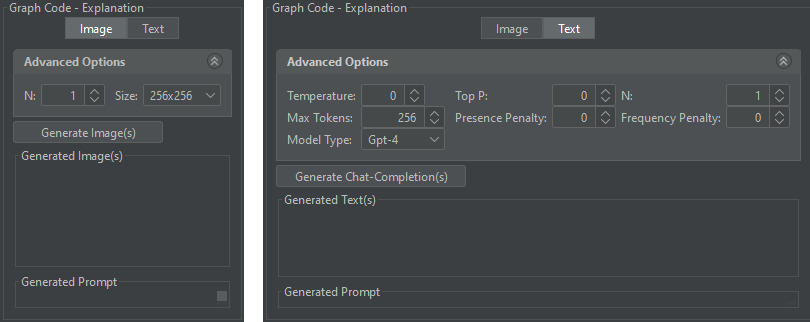
\includegraphics[width=\textwidth]{chapter/chapter_5/new-layouts-img-txt}
  \caption[Umordnung der Layouts von \textit{ImagePanel} und \textit{TextPanel}]{Umordnung der Layouts von \textit{ImagePanel} (links) und \textit{TextPanel} (rechts).}
  \label{sec5:eval:subsec:adaptation:fig:new-layouts}
\end{figure}

Das Beheben des dritten Mangels erfordert eine umfassendere Anpassung der Benutzeroberfläche, sowie eine Anpassung der Verarbeitung der generierten Ergebnisse.
Anstatt eines Labels zur Darstellung des generierten Bildes, bzw. eines Textfeldes zur Darstellung des generierten Textes, müssen nun mehrere Darstellungen in einer Benutzungsschnittstelle eingebunden werden.
Hierfür wird auf ein Registerkartenpanel \textit{JTabbedPane} anstelle des Labels \textit{JLabel} bzw. des Textfeldes \textit{JTextArea} zurückgegriffen.
Dieses Registerkartenpanel bietet das Darstellen mehrere Registerkarten mit eigenständigem Inhalt, sowie dem Hin- und Herschalten zwischen diesen Registerkarten.
Die Komponenten zur Darstellung der Inhalte bleiben unverändert ein \textit{JLabel} bzw. eine \textit{JTextArea}, die nun allerdings als Registerkarten dem Registerkartenpanel dynamisch hinzugefügt werden.
Das dynamische Hinzufügen erfolgt durch eine Anpassung der Verarbeitung, die in Bezug auf die Ergebnisse vorsieht, dass alle Datenelemente bzw. Inhalte einer Antwort durchlaufen werden.
\cref{sec5:eval:subsec:adaptation:fig:tabbedpane-image} zeigt die Darstellung mehrerer Registerkarten mit generierten Bildern in einem Registerkartenpanel in der Benutzungsschnittstelle \textit{ImagePanel}.

\begin{figure}[!ht]
  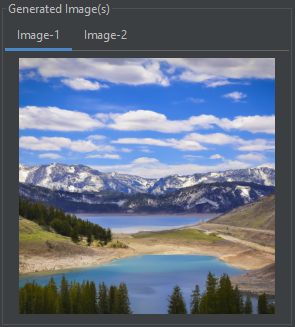
\includegraphics{chapter/chapter_5/tabbedpane-image}
  \caption{Registerkartenpanel in der Benutzungsschnittstelle \textit{ImagePanel} mit zwei Registerkarten.}
  \label{sec5:eval:subsec:adaptation:fig:tabbedpane-image}
\end{figure}

Das Beheben des letzten Mangels erfolgt durch das Modifizieren der Darstellung des Mauszeigers.
Eine geeignete Darstellung für einen Mauszeiger, der einen laufenden Hintergrundprozess darstellen soll, ist eine Sanduhr.
Die Modifikation dieser Darstellung kann in den entsprechenden Benutzungsschnittstellen \textit{ImagePanel} oder \textit{TextPanel} durch die Methode \textit{setCursor(...)} erfolgen.
In dem Moment, in dem ein Benutzer den Knopf \enquote{Generate ...} betätigt, wird im Hintergrund ein entsprechender Arbeitsprozess zum Generieren einer Erklärung begonnen und der Mauszeiger wird zu einer Sanduhr angepasst.
Sobald der Arbeitsprozess abgeschlossen wurde, erfolgreich oder nicht, wird der Mauszeiger auf den Standardwert zurückgesetzt.

Unabhängig von diesen Mängeln schlägt der Experte eine optionale Erweiterung der Benutzungsschnittstelle vor.
Um den Benutzern der Anwendung eine besseres Einordnen bzw. ein besseres in Bezug setzen der generierten Erklärungen zu den ursprünglichen Dateien zu ermöglichen, schlägt der Experte das Umsetzen einer Gegenüberstellung des entsprechenden Graph Codes, der Original-Datei und der generierten Erklärung vor.
Diese Gegenüberstellung wird erreicht durch das Hinzufügen einer Registerkartenpanels im rechten Teil des Grundbereichs \textit{EditorGraphCode} mit entsprechenden Registerkarten.
Diese Registerkarten sind zum einen die tabellarische Darstellung des Graph Codes, \textit{GraphCodeTable} und zum anderen eine neue Benutzungsschnittstelle \textit{OriginalAssetPanel}, die anhand des Dateinamens einer Graph Code Datei in der Kollektion nach einer entsprechenden Datei sucht und diese geeignet darstellt.
Hierfür kann zum Großteil auf bereits bestehenden Quellcode der Komponente \textit{AssetDetailPanel} zurückgegriffen werden.
\cref{sec5:eval:subsec:adaptation:fig:original-asset} zeigt die neue Benutzungsschnittstelle \textit{OriginalAssetPanel} zum Darstellen der originalen Datei.
Eine komplette Gegenüberstellung einer generierten visuellen Erklärung zu ihrer entsprechenden originalen Datei kann in \cref{sec5:eval:subsec:adaptation:fig:gc-orig-exp} eingesehen werden.

\begin{figure}[!ht]
  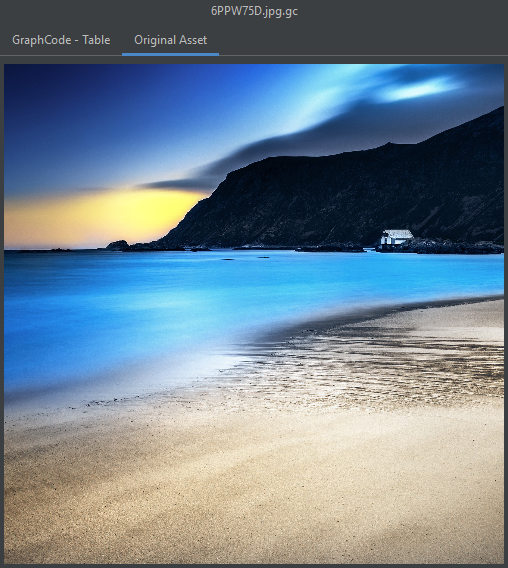
\includegraphics{chapter/chapter_5/original-asset}
  \caption{Ausgewählte Registerkarte mit der Darstellung der mit einem Graph Code ursprünglich assoziierten Datei.}
  \label{sec5:eval:subsec:adaptation:fig:original-asset}
\end{figure}

\begin{figure}[!ht]
  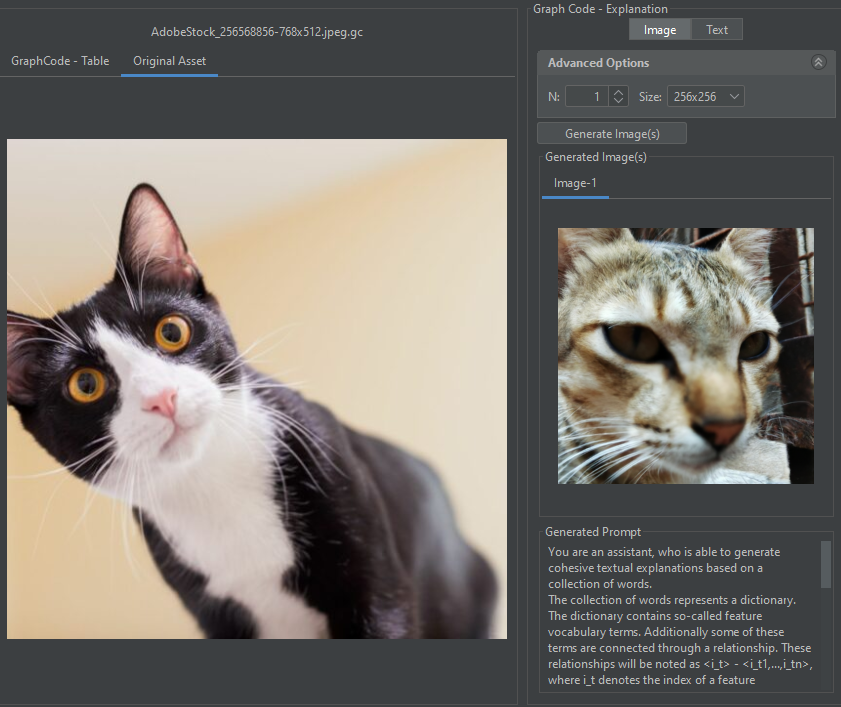
\includegraphics[width=\textwidth]{chapter/chapter_5/gc-orig-exp}
  \caption{Gegenüberstellung eines Graph Codes, der originalen Datei und der erzeugten visuellen Erklärung.}
  \label{sec5:eval:subsec:adaptation:fig:gc-orig-exp}
\end{figure}

Im Folgenden werden noch weitere Anpassungen an der prototypischen Proof-of-Concept Implementierung beschrieben, die unabhängig von den in der Evaluierung durchgeführten Experimenten erfolgten.

Im Umgang mit generativer KI sind Tokens von großer Bedeutung.
Es wurde daher in der Benutzungsschnittstelle \textit{TextPanel} eine Informationsoberfläche hinzugefügt, die es einem Benutzer ermöglicht, die Tokenanzahl eines generierten Textes einzusehen.
Darüber hinaus können durch diese Informationsoberfläche die Tokens in jenem Text farbig hervorgehoben werden.
Diese Anpassung kann \cref{sec5:eval:subsec:adaptation:fig:custom-token-info} eingesehen werden.

\begin{figure}[!ht]
  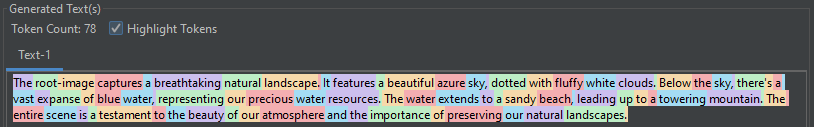
\includegraphics[width=\textwidth]{chapter/chapter_5/custom-token-info}
  \caption{Informationsoberfläche für Tokens in einem generierten Text.}
  \label{sec5:eval:subsec:adaptation:fig:custom-token-info}
\end{figure}

Eine weitere Anpassung, die eine sinnvolle Erweiterung der Funktionen der Anwendung darstellt, ist das automatische Sichern der in der Benutzungsschnittstelle \textit{ImagePanel} generierten Bilder in einem dafür vorgesehenen Ordner \enquote{explanations}.

% So wurde von OpenAI zum Zeitpunkt des Verfassens dieser Arbeit eine neue Version von Dall-E, Dall-E 3 \cite{dall-e-3}, vorgestellt, welches eine erhebliche Verbesserung zu vorherigen Systemen darstellen soll \cite{dall-e-3-paper}.

Infolge des angekündigten Updates \cite{openai-new-update-6_11_23} von OpenAI am 6. November 2023 (OpenAI DevDay \cite{openai-dev-day}) konnten weitere Anpassungen und Erweiterungen an der entwickelten Anwendung vorgenommen werden.
Dieses Update umfasst eine Reihe an Verbesserungen, Anpassungen und Erweiterungen.
Zu den Erweiterungen gehören die neue Dall-E 3 Schnittstelle, sowie eine Text-To-Speech (TTS, z.Dt. Text zu Sprache) Schnittstelle, mit welcher eine Audiodatei bzw. ein clip für einen beliebigen Text generiert werden kann.
Diese Neuerungen wurden ausgewählt und in die Anwendung integriert.
Die Integration dieser Erweiterungen äußert sich in einer Anpassung der Benutzungsschnittstelle \textit{ImagePanel} des Erklärungstyps Bild, welches hauptsächlich neue Auswahlmöglichkeiten in den erweiterten Optionen umfasst, sowie durch eine neue Benutzungsschnittstelle \textit{AudioPanel}, einsehbar in \cref{sec5:eval:subsubsec:adaptation:fig:audio-ui}, für einen neuen Erklärungstyp Audio, mit welchem auditive Erklärungen in Form von (kurzen) Audiodateien bzw. clips zu Graph Codes generiert werden können.
Aufgrund der Größe der durch Dall-E 3 generierten Bilder (1024x1024, 1792x1024, 1024x1792) können diese nicht mehr in der Benutzungsschnittstelle angezeigt werden und es wird stattdessen ein Knopf zum Öffnen des Bildes in einem externen Fenster angeboten.

\begin{figure}[!ht]
  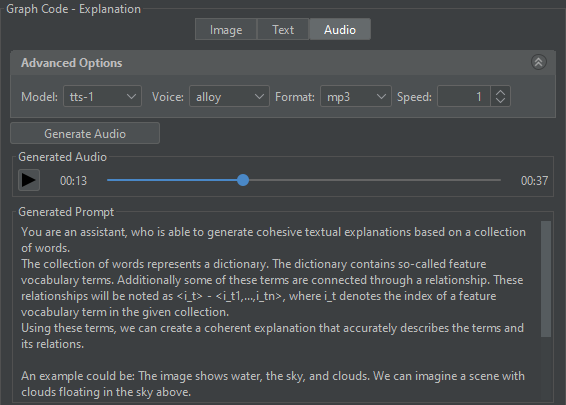
\includegraphics{chapter/chapter_5/right_audio_exp}
  \caption{Benutzungsschnittstelle für den Erklärungstyp Audio.}
  \label{sec5:eval:subsubsec:adaptation:fig:audio-ui}
\end{figure}

\clearpage

\subsection{Zusammenfassung}
\label{sec5:eval:subsec:summary}
Inhalt dieses Kapitels war die Evaluierung der im Rahmen der Implementierung entwickelten prototypischen Proof-of-Concept Implementierung.
In \cref{sec5:eval:subsec:eval-goals-methodology} wurden zuerst die Ziele der Evaluierung formuliert.
In Vorbereitung der Evaluierung wurden dann in \cref{sec5:eval:subsec:assign-exper} Aufgaben bzw. Experimente formuliert, die aus den Anwendungsfällen in \cref{sec3:model} abgeleitet wurden.
Diese Experimente wurden dann, der Methodik nach Nunamaker entsprechend, den Forschungszielen zugewiesen.
In den Forschungszielen FZ 1.4/E und FZ 2.4/E wurde dann jeweils die Vorbereitung, die Durchführung und die Einordnung der Ergebnisse des jeweiligen Experiments behandelt.
Die in diesen Forschungszielen gesammelten Erkenntnisse umfassen in erster Linie eine Reihe an Mängeln, die in der Durchführung der jeweiligen Experimente identifiziert werden konnten.
Als Reaktion auf diese Mängel wurden dann in \cref{sec5:eval:subsec:adaptation} Anpassungen an der Benutzungsschnittstelle und Funktionen der Anwendung beschrieben.

\subsubsection{Gewonnene Erkenntnisse}
In diesem Abschnitt werden die Erkenntnisse aus den Forschungszielen \enquote{FZ 1.4/E Erklärbarkeit von MMIR mittels generativer KI} und \enquote{FZ 2.4/E Integration generativer KI in das GMAF} zusammengefasst.

% Erkenntnisse aus FZ 1.4/E sammeln bzw. noch einmal kurz darstellen... (Hier auch die definierten Ziele der Evaluierung aufgreifen)
% Wurden Aspekte wie Vollständigkeit und Korrektheit durch die Evaluierungsmethodik abgedeckt und zu welchem Schluss kommt man nach der Durchführung des jeweiligen Experiments...?

In \cref{sec5:eval:subsec:fz-explainability} \enquote{FZ 1.4/E Erklärbarkeit von MMIR mittels generativer KI} konnte durch die Durchführung des Experiments \textbf{Exp. 1} festgestellt werden, dass die Anwendung eine Reihe an nicht fatalen Mängeln aufweist.
Nicht fatal soll ausdrücken, dass diese Mängel die Funktionen und Abläufe in dem Programm nicht negativ beeinträchtigen, sodass Benutzer der Anwendung ihre formulierten Ziele erreichen können.
Allerdings beeinträchtigen diese Mängel durchaus die Intuivität bzw. den Umgang mit dem Programm.
Zum Abschluss des Experiments wurden diese Mängel gesammelt, beschrieben und jeweils potentielle Lösungsvorschläge formuliert.
Auf die Ziele der Evaluierung rückblickend konnte festgehalten werden, dass beide Ziele, Vollständigkeit und Korrektheit der Implementierung, zufriedenstellend erfüllt wurden.

% Erkenntnisse aus FZ 2.4/E sammeln bzw. noch einmal kurz darstellen... (Hier auch die definierten Ziele der Evaluierung aufgreifen)
% Wurden Aspekte wie Vollständigkeit und Korrektheit durch die Evaluierungsmethodik abgedeckt und zu welchem Schluss kommt man nach der Durchführung des jeweiligen Experiments...?

In \cref{sec5:eval:subsec:fz-integration} \enquote{FZ 2.4/E Integration generativer KI in das GMAF} konnte durch die Durchführung des Experiments \textbf{Exp. 2} festgestellt werden, dass die Anwendung eine Reihe an nicht fatalen Mängeln aufweist.
Auch diese Mängel betreffen nicht die Funktionen und Abläufe des Programms, sondern beeinträchtigen nur die Intuivität bzw. den Umgang mit dem Programm.
Zum Abschluss des Experiments wurden diese Mängel gesammelt, beschrieben und jeweils potentielle Lösungsvorschläge formuliert.
Auf die Ziele der Evaluierung rückblickend konnte festgehalten werden, dass beide Ziele, Vollständigkeit und Korrektheit der Implementierung, zufriedenstellend erfüllt wurden.

Infolge der in den Experimenten identifizierten Mängel und den darauffolgend beschriebenen Lösungsvorschlägen wurden in \cref{sec5:eval:subsec:adaptation} Anpassungen an der prototypischen Proof-of-Concept Implementierung beschrieben, um diese Mängel zu beseitigen.
Diese Anpassungen variieren stark in ihrem Umfang, betreffen aber in erster Linie nur den Aufbau oder die Interaktion mit der Benutzungsschnittstelle.
Da keine fatalen Mängel festgestellt werden konnten, mussten keine Anpassungen an Datenmodell bezogene Algorithmen vorgenommen werden.

Darüber hinaus wurden, unabhängig von den in den Experimenten identifizierten Mängeln, in \cref{sec5:eval:subsec:adaptation} weitere Anpassungen und Erweiterungen von Funktionen der Anwendung beschrieben, die vom Experten vorgeschlagen oder vom Autor als sinnvoll erachtet wurden.

Aufgrund mangelnder Ressourcen konnte im Rahmen der Evaluierung keine umfassendere Prüfung der prototypischen Anwendung auf Fehler und Defekte durchgeführt werden.
Daher wurde mit den verfügbaren Ressourcen eine andere Evaluierungsmethodik durchgeführt, nach welchem für die Evaluierung festgehalten werden kann, dass die in dieser Arbeit entwickelte prototypische Proof-of-Concept Implementierung eine funktionierende Anwendung darstellt und welche das übergeordnete Ziel, Erklärungen von Graph Codes mittels generativer KI zu erzeugen, zufriedenstellend erfüllt.

Die nachfolgende Tabelle stellt eine Erweiterung der \cref{sec4:impl:subsec:summary:table:summary} dar und gibt eine Übersicht über den aktuellen Arbeitsstand nach Abschluss dieses Kapitels.

\begingroup
\def\arraystretch{1.1}%
\begin{xltabular}{\linewidth}{
            @{}
            >{
                \hsize=0.2\linewidth
                \raggedright\arraybackslash
            }X
            >{
                \hsize=0.6\linewidth
                \raggedright\arraybackslash
            }X
            >{
                \hsize=0.2\linewidth
            }X
            @{}
        }

        % First Header

        \caption{Tabelle zur Übersicht des aktuellen Arbeitsstands.}
        \label{sec5:eval:subsec:summary:table:summary}
        \\

        \toprule
        \multicolumn{3}{
            >{
                    \hsize=\linewidth\centering\arraybackslash
            }X
        }
        {
            \textbf{Forschungsziele}
        } \\ \midrule
        \textbf{FZ / OH} &  \textbf{Beschreibung} & \textbf{Referenz} \\ \midrule

        \endfirsthead

        \toprule
        \multicolumn{3}{
            >{
                    \hsize=\linewidth\centering\arraybackslash
            }X
        }
        {
            \textbf{Forschungsziele}
        } \\ \midrule
        \textbf{FZ / OH} & \textbf{Beschreibung} & \textbf{Referenz} \\ \midrule

        \endhead

        % Lower Rows

        \multicolumn{3}{
            >{
                    \hsize=\linewidth\centering\arraybackslash
            }X
        }
        {
            \textbf{Erklärbarkeit von MMIR mittels generativer KI}
        }
        \\
        \midrule

        FZ 1.1/O
        &
        Recherche zur Erklärbarkeit von MMIR mittels generativer KI
        \\

        &
        Grundlegende Technologien:
        &

        \\

        &
        \tabitem GMAF
        &
        \cref{sec2:sota:subsubsec:gmaf}
        \\

        &
        \tabitem MMFG
        &
        \cref{sec2:sota:subsubsec:mmfg}
        \\

        &
        \tabitem Graph Code
        &
        \cref{sec2:sota:subsubsec:graph-codes}
        \\

        % Offene Herausforderungen aus FZ1/O

        OH 1.1
        &
        Erste offene Herausforderung
        &
        \hyperref[sec2:sota:oi:1.1]{\textbf{OH 1.1}}
        \\


        &
        Systeme generativer KI und ein Überlick über aktuelle Systeme
        &
        \cref{sec2:sota:subsubsec:genai}
        \\

        &
        Diskussion und Auswahl von Systemen
        &
        \cref{sec2:sota:subsubsec:fz1:discussion}
        \\

        OH 1.2
        &
        Zweite offene Herausforderung
        &
        \hyperref[sec2:sota:oi:2.1]{\textbf{OH 2.1}}
        \\

        \midrule

        FZ 1.2/TB
        &
        Modellierung der Erklärbarkeit von MMIR mittels generativer KI
        &

        \\

        &
        Erklärbarkeit durch generative KI
        &
        \cref{sec3:model:subsubsec:explainability-through-genai}
        \\

        &
        $\rightarrow$ Behandlung der ersten offenen Herausforderung \hyperref[sec2:sota:oi:1.1]{\textbf{OH 1.1}}
        &
        \\

        &
        Anwendungsfälle:
        &
        \cref{sec3:model:subsubsec:use-cases}
        \\

        &
        \tabitem Textuelle Beschreibungen
        &
        %\cref{sec3:model:par:textual-desc-use-cases}
        \\

        &
        Wireframes
        &
        \cref{sec3:model:par:wireframe}
        \\

        &
        Mechanismen
        &
        \cref{sec3:model:par:mechanism-use-cases}
        \\

        &
        Sequenzdiagramme
        &
        \cref{sec3:model:par:seq-use-cases}
        \\

        &
        $\rightarrow$ Behandlung der zweiten offenen Herausforderung \hyperref[sec2:sota:oi:1.2]{\textbf{OH 1.2}}
        &
        \\

        \midrule

        FZ 1.3/I
        &
        Implementierung der Erklärbarkeit von MMIR mittels generativer KI
        &

        \\

        &
        Benutzungsschnittstelle:
        &
        \cref{sec4:impl:subsubsec:ui}
        \\

        &
        \tabitem Elemente der Benutzeroberfläche
        &
        \\

        &
        \tabitem Interaktion mit der Benutzeroberfläche
        &
        \\

        \midrule

        FZ 1.4/E
        &
        Evaluierung der Erklärbarkeit von MMIR mittels generativer KI
        &

        \\

        &
        Experiment \textbf{Exp. 1}:
        &
        \\

        &
        \tabitem Vorbereitung des Experiments
        &
        \cref{sec5:eval:subsubsec:exp-1:preparation}
        \\

        &
        \tabitem Durchführung des Experiments
        &
        \cref{sec5:eval:subsubsec:exp-1:execution}
        \\

        &
        \tabitem Erkenntnisse des Experiments
        &
        \cref{sec5:eval:subsubsec:exp-1:results-discussion}
        \\

        \midrule

        \multicolumn{3}{
            >{
                    \hsize=\linewidth\centering\arraybackslash
            }X
        }
        {
            \textbf{Integration generativer KI in das GMAF}
        }
        \\
        \midrule

        FZ 2.1/O
        &
        Recherche zur Integration generativer KI in das GMAF
        &

        \\


        &
        Aufzeigen der Integrationsmöglichkeiten von:
        &

        \\

        &
        \tabitem Graph Codes
        &
        \cref{sec2:sota:subsubsec:gc-capabilities-integration}
        \\

        &
        Erste offene Herausforderung
        &
        \hyperref[sec2:sota:oi:2.1]{\textbf{OH 2.1}}
        \\

        &
        \tabitem Systemen generativer KI
        &
        \cref{sec2:sota:subsubsec:genai-capabilities-integration}
        \\

        &
        Zweite offene Herausforderung
        &
        \hyperref[sec2:sota:oi:2.2]{\textbf{OH 2.2}}
        \\

        \midrule

        FZ 2.2/TB
        &
        Modellierung der Integration generativer KI in das GMAF
        &

        \\

        &
        Transformation von Graph Codes
        &
        \cref{sec3:model:subsubsec:gc-transformation}
        \\

        &
        \tabitem Transformation des Vokabulars
        &
        \\

        &
        \tabitem Transformation der Matrix
        &
        \\

        &
        \tabitem Anwendung von Graph Code Metriken
        &
        \\

        &
        $\rightarrow$ Behandlung der ersten offenen Herausforderung \hyperref[sec2:sota:oi:2.1]{\textbf{OH 2.1}}
        &
        \\

        &
        Einbindung generativer KI in das GMAF
        &
        \cref{sec3:model:subsubsec:genai-integration}
        \\

        &
        $\rightarrow$ Behandlung der zweiten offenen Herausforderung \hyperref[sec2:sota:oi:2.2]{\textbf{OH 2.2}}
        &
        \\

        \midrule

        FZ 2.3/I
        &
        Implementierung der Integration generativer KI in das GMAF
        &

        \\

        &
        Transformation von Graph Codes
        &
        \cref{sec4:impl:subsubsec:gc-transformation}
        \\

        &
        Integration der Endpunkte
        &
        \cref{sec4:impl:subsubsec:endpoint-integration}
        \\

        \midrule

        FZ 2.4/E
        &
        Evaluierung der Integration generativer KI in das GMAF
        &

        \\

        &
        Experiment \textbf{Exp. 2}:
        &
        \\

        &
        \tabitem Vorbereitung des Experiments
        &
        \cref{sec5:eval:subsubsec:exp-2:preparation}
        \\

        &
        \tabitem Durchführung des Experiments
        &
        \cref{sec5:eval:subsubsec:exp-2:execution}
        \\

        &
        \tabitem Erkenntnisse des Experiments
        &
        \cref{sec5:eval:subsubsec:exp-2:results-discussion}
        \\

        \bottomrule
\end{xltabular}
\endgroup


Im nächsten \cref{sec6:disc} \enquote{Zusammenfassung} wird die gesamte Arbeit zusammengefasst, auf die Forschungsfragen aus dem ersten Kapitel zurückgesprungen und weitere Informationen in Bezug auf diese Arbeit beschrieben.
